%Template for PhD reports By: Roberto Contreras
% Modified by: Aminadab Córdova 
% Last update: 2025-03-24
%Comment out two column if need two column writing

\documentclass[11pt]{article}
%\documentclass[11pt, twocolumn]{report}

%Package to generate latin text (Only for testing)
\usepackage{lipsum}

\usepackage{amsmath}
\usepackage{amsfonts}
\usepackage{amssymb}
%AMS packages for mathematical symbols

%package to include pictures and images
\usepackage{graphicx}

%Package to setup page layout
\usepackage[margin=1in, includefoot, includehead]{geometry}

%Uses hyperlinks in PDF (optional)
\usepackage[hidelinks]{hyperref}

%Header and Footer Stuff
\usepackage{fancyhdr}
\pagestyle{fancy}
\fancyhead{}
\fancyfoot{}
\fancyhead[R]{\myTitle}
\fancyfoot[L]{Maestría en Inteligencia Artificial y Analítica de Datos}
\fancyfoot[R]{\thepage}
\renewcommand{\footrulewidth}{1pt}

%Package to get current date
\usepackage{datetime}


%bibliography packages
\usepackage{natbib}  % Para manejar citas con BibTeX
% \usepackage{hyperref}   Para hipervínculos en la bibliografía

\usepackage[utf8]{inputenc} % Codificación UTF-8
\usepackage[T1]{fontenc}    % Codificación de fuentes
\usepackage[spanish]{babel} % Idioma español
\usepackage{xcolor}         % Colores
\usepackage{listings}       % Para mostrar código fuente

% ===== Configuración de estilos para Python =====
\definecolor{codegreen}{rgb}{0,0.6,0}
\definecolor{codegray}{rgb}{0.5,0.5,0.5}
\definecolor{codepurple}{rgb}{0.58,0,0.82}
\definecolor{backcolour}{rgb}{0.95,0.95,0.92}

\lstdefinestyle{mypython}{
    language=Python,
    backgroundcolor=\color{backcolour},
    commentstyle=\color{codegreen},
    keywordstyle=\color{magenta},
    numberstyle=\tiny\color{codegray},
    stringstyle=\color{codepurple},
    basicstyle=\ttfamily\footnotesize,
    breaklines=true,
    frame=single,
    captionpos=b,
    numbers=left,
    numbersep=5pt,
    showspaces=false,
    showstringspaces=false,
    showtabs=false,
    literate={á}{{\'a}}1 {é}{{\'e}}1 {í}{{\'i}}1 {ó}{{\'o}}1 {ú}{{\'u}}1
             {Á}{{\'A}}1 {É}{{\'E}}1 {Í}{{\'I}}1 {Ó}{{\'O}}1 {Ú}{{\'U}}1
             {ñ}{{\~n}}1 {Ñ}{{\~N}}1
             {“}{{``}}1 {”}{{''}}1 {‘}{{`}}1 {’}{{'}}1
}


% Document Variables 
\newcommand{\myTitle}{Reporte de práctica \\ El problema de despacho económico de carga}
\newcommand{\myName}{Alumno: Aminadab Córdova Acosta}
\newcommand{\myClass}{Asignatura: Programación para Analítica Prescriptiva y de Apoyo a la Decisión}
\newcommand{\myTecher}{Instructor: Dr. Josué Domínguez Guerrero}
\newcommand{\myDate}{\today}  % This will insert the current date

%Document Start
\begin{document}

\begin{titlepage}
    \begin{center}
        
\includegraphics[scale=0.75]{UACJ.png}\\
        \huge{\textbf{Universidad Autónoma\\de Ciudad Juárez}} \\ 
        [0.25in] 
        
        \textbf{\Large{Instituto de Ingeniería y Tecnología}}\\
        \Large{Departamento de Ingeniería Eléctrica y Computación}\\
        \Large{Maestría en Inteligencia Artificial y Analítica de Datos}\\
        [1in]

        \line(1,0){400}\\
        [2mm]
        \textsc{\Large{\myTitle}} \\ 
        \line(1,0){400} \\ 
        [1in]
    \end{center}
    \begin{center}
        \myName \\ 
        \myClass\\ 
        \myTecher\\
        [0.5in]
        \myDate
    \end{center}
\end{titlepage}

%If need adding sections, please uncomment next lines
%Before TOC
\pagenumbering{roman}
\section*{Resumen}
\addcontentsline{toc}{section}{\numberline{}Resumen}
Este reporte presenta la resolución de un caso práctico de Despacho Económico de Carga utilizando Pyomo en Python. Se formula un modelo de optimización no lineal para minimizar el costo de generación, asegurando el cumplimiento de restricciones técnicas y operativas. La resolución se lleva a cabo con el solver IPOPT, especializado en optimización no lineal. Finalmente, se interpretan los resultados del modelo, destacando su impacto en la toma de decisiones dentro del sistema eléctrico.
\cleardoublepage

%If need table of contents, please uncomment next lines
%Table of contents
\tableofcontents
\thispagestyle{empty}
\cleardoublepage

%Start your text here
\pagenumbering{arabic} % Start numbering pages from 1
\setcounter{page}{1}   % Ensure the page counter starts at 1

\section{Introducción}	
El problema de despacho económico de carga consiste en determinar la cantidad de potencia que deben suministrar las unidades de generación a la red eléctrica, de manera que se cubra la demanda total de energía al menor costo posible, cumpliendo al mismo tiempo con las restricciones técnicas y operativas del sistema \citep{en17030550}.

La optimización juega un papel fundamental en este proceso, ya que el despacho económico se plantea como un problema matemático en el que se busca minimizar el costo total de generación, sujeto a diversas restricciones económicas y técnicas del sistema eléctrico \citep{osti_6202356}.

En este trabajo se replica el caso de estudio del sistema 1 presentado en \citep{electronics9010108}, donde se formula un modelo de despacho económico de carga, ilustrado en la Figura 1 y se resuelve utilizando Pyomo, una biblioteca de optimización en Python. Los datos del sistema se toman de esta referencia. Se presenta una descripción detallada del problema, la formulación matemática del modelo, la implementación en Pyomo, y la interpretación de los resultados obtenidos.

\newpage
\section{Descripción general del caso de estudio}

El caso de estudio se centra en un sistema eléctrico compuesto por seis unidades generadoras ilustrado en la Fig. 1, cada una con características técnicas y económicas específicas. El objetivo principal es determinar la asignación óptima de potencia generada por cada unidad, minimizando el costo total de generación mientras se cumplen las restricciones operativas y técnicas del sistema.

El sistema considera los siguientes aspectos clave que se encuentran en la Tabla 4 y el apéndice A de \citep{electronics9010108}:
\begin{itemize}
    \item \textbf{Restricciones de generación:} Cada unidad generadora tiene límites mínimos y máximos de potencia que deben respetarse.
    \item \textbf{Restricciones de rampa:} Las unidades generadoras tienen límites en la velocidad de cambio de potencia entre periodos consecutivos.
    \item \textbf{Pérdidas de transmisión:} Se incluyen pérdidas de transmisión en las líneas eléctricas, modeladas mediante una matriz de coeficientes \( B \).
    \item \textbf{Demanda total:} La generación total debe satisfacer la demanda del sistema (1263 MW), considerando las pérdidas de transmisión.
    \item \textbf{Costos de generación:} Los costos de generación de cada unidad se modelan como funciones cuadráticas, con términos adicionales para representar efectos no lineales como el punto de válvula.
\end{itemize}

\begin{figure}[h!]
    \centering
    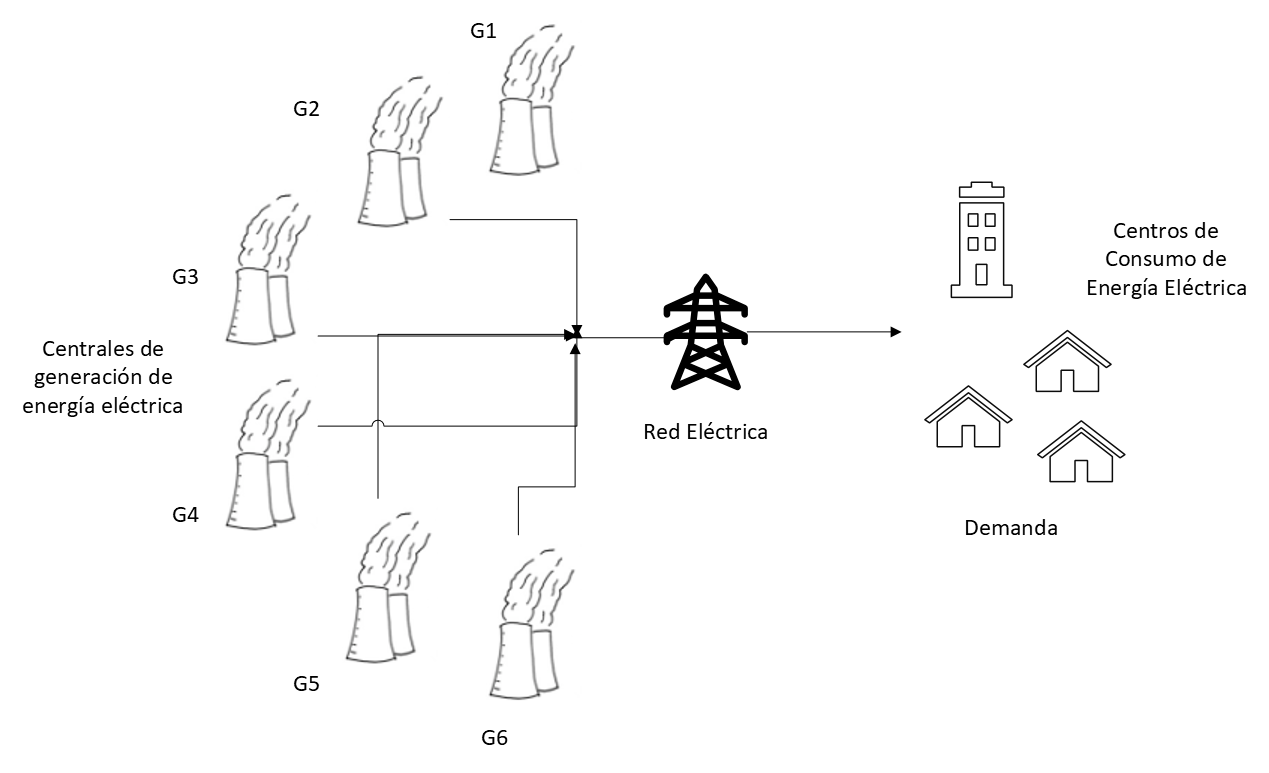
\includegraphics[width=0.8\textwidth]{economic-dispatch.png}
    \caption{Representación del problema de despacho económico de carga.}
    \label{fig:economic_dispatch}
\end{figure}

\newpage
\section{Modelo matemático}
\subsection{Función Objetivo}

Al asignar razonablemente la producción de las unidades, los costos operativos pueden reducirse significativamente. 
El modelo de costos se simplifica a continuación:

\begin{equation}
    \min (F_T) =\min  \sum_{i=1}^{N} F_i(P_{Gi})
\end{equation}

Donde \( F_T \) indica el costo total del combustible, \( N \) representa el numero total de unidades de generación, 
\( P_{Gi} \) es la salida de potencia activa del \( i \)-th generador, y \( F_i(P_{Gi}) \) significa el costo del consumo 
de combustible correspondiente del \( i \)-th generador, y se puede expresar como un polinomio cuadrático dependiente de 
la potencian:

\begin{equation}
    F_i(P_{Gi}) = a_i(P_{Gi})^2 + b_i(P_{Gi}) + c_i
\end{equation}

donde \( a_i \), \( b_i \), and \( c_i \) representan los coeficientes de costo del combustible. Cuando la válvula de 
admisión de la turbomáquina se abre repentinamente, el resultado, conocido como 'efecto de punto de válvula', 
puede representarse generalmente como una función sinusoidal. Esta función sinusoidal se añadirá a la tradicional 
función de costo de combustible cuadrática, es decir:

\begin{equation}
    F_i(P_{Gi}) = a_i(P_{Gi})^2 + b_i(P_{Gi}) + c_i + |d_i \sin(e_i (P_{Gi}^{\min} - P_{Gi}))|
\end{equation}

Donde \( P_{Gi}^{\min} \) representa el límite inferior de la potencia de salida del \( i \)-th generador, 
y \( |d_i| \) y \( e_i \) son los coeficientes de costo. 

\subsection{Restricciones de Balance de Potencia}
Las restricciones de equilibrio de potencia son las restricciones más críticas en la operación de la unidad generadora. 
Si no se cumple esta restricción, se producirá la parálisis del sistema eléctrico y se amenazará seriamente la fiabilidad
 de la operación del sistema. Esta restricción se puede resumir en que la producción total de todas las unidades generadoras 
 debe ser igual a la suma de la carga y la pérdida de transmisión

\begin{equation}
    \sum_{i=1}^{N} P_{Gi} = P_{D} + P_{L}
\end{equation}

\begin{equation}
    P_{L} = \sum_{i=1}^{N}\sum_{j=1}^{N} P_{Gi}B_{ij}P_{Gj} + \sum_{i=1}^{N}B_{i0}P_{Gi} + B_{00}
\end{equation}

\subsection{Restricciones de Generación}

La potencia de salida de cada generador debe estar dentro de los límites de generación, es decir:

\begin{equation}
    P_{Gi}^{\min} \leq P_{Gi} \leq P_{Gi}^{\max}
\end{equation}

donde \( P_{Gi}^{\min} \) y \( P_{Gi}^{\max} \) son los límites inferior y superior de la potencia de salida del 
\( i \)-th generador, respectivamente.

\subsection{Límite de velocidad de rampa}
%La capacidad de rampa de cada generador debe estar dentro de los límites de rampa, es decir:

%\begin{equation}
    %\Delta P_{Gi}^{\min} \leq \Delta P_{Gi} \leq \Delta P_{Gi}^{\max}
%\end{equation}

Dentro de un período de tiempo, la variación de potencia está limitada por el funcionamiento del generador. 
Esta restricción se describe a continuación:

\begin{equation}
    - DR_{i} \leq  P_{Gi} - P_{Gi(t-1)} \leq UR_{i}
\end{equation}

Donde \( DR_{i} \) y \( UR_{i} \) son las tasas de disminución y aumento de potencia del \( i \)-th generador,
respectivamente.

\subsection{Límites de las zonas de operación prohibida}

La potencia de salida de cada generador debe estar fuera de las zonas de operación prohibida, es decir:

\begin{equation}
    P_{Gi}^{\min} \leq P_{Gi} \leq P_{Gi}^{\max}
\end{equation}

Los cojinetes del generador producirán vibraciones intensas cuando el generador funcione en algunas
zonas. Por lo tanto, la potencia de salida debe ajustarse para evitar zonas de funcionamiento prohibidas durante
la operación real. Los límites de las zonas de funcionamiento prohibidas se enumeran a continuación:

\begin{equation}
    \left\{
    \begin{array}{l}
        P_{Gi}^{\min} \leq P_{Gi} \leq P_{Gi}^{1} \\[8pt]
        P_{Gi}^{k-1} \leq P_{Gi} \leq P_{Gi}^{k}, \quad k = 2,3,\dots,n_Z \\[8pt]
        P_{Gi}^{n_Z} \leq P_{Gi} \leq P_{Gi}^{\max}
    \end{array}
    \right.
\end{equation}

\newpage
\section{Código en Python}
El modelo matemático presentado anteriormente se implementa en Pyomo, una biblioteca de optimización en Python. Pyomo permite definir modelos de optimización de manera sencilla y eficiente, y proporciona una interfaz para resolverlos con diversos solvers. A continuación se presenta la implementación del modelo de despacho económico de carga en Pyomo.

\begin{lstlisting}[style=mypython, caption={Modelo de Despacho Económico con Pyomo}]
from pyomo.environ import *
    
# Crear el modelo
model = ConcreteModel()
    
# Conjunto de generadores
model.Generadores = Set(initialize=['G1', 'G2', 'G3', 'G4', 'G5', 'G6'])
    
# Parámetros de los generadores
datos_generadores = {
    'G1': {'Pmax': 500, 'Pmin': 100, 'ai': 0.007, 'bi': 7, 'ci': 240, 'UR': 80, 'DR': 120, 'Pi': 440},
    'G2': {'Pmax': 200, 'Pmin': 50, 'ai': 0.0095, 'bi': 10, 'ci': 200, 'UR': 50, 'DR': 90, 'Pi': 170},
    'G3': {'Pmax': 300, 'Pmin': 80, 'ai': 0.009, 'bi': 8.5, 'ci': 220, 'UR': 65, 'DR': 100, 'Pi': 200},
    'G4': {'Pmax': 150, 'Pmin': 50, 'ai': 0.009, 'bi': 11, 'ci': 200, 'UR': 50, 'DR': 90, 'Pi': 150},
    'G5': {'Pmax': 200, 'Pmin': 50, 'ai': 0.008, 'bi': 10.5, 'ci': 220, 'UR': 50, 'DR': 90, 'Pi': 190},
    'G6': {'Pmax': 120, 'Pmin': 50, 'ai': 0.0075, 'bi': 12, 'ci': 190, 'UR': 50, 'DR': 90, 'Pi': 110}
}
    
# Definir parámetros en el modelo
model.Pmax = Param(model.Generadores, initialize={g: datos_generadores[g]['Pmax'] for g in model.Generadores})
model.Pmin = Param(model.Generadores, initialize={g: datos_generadores[g]['Pmin'] for g in model.Generadores})
model.ai = Param(model.Generadores, initialize={g: datos_generadores[g]['ai'] for g in model.Generadores})
model.bi = Param(model.Generadores, initialize={g: datos_generadores[g]['bi'] for g in model.Generadores})
model.ci = Param(model.Generadores, initialize={g: datos_generadores[g]['ci'] for g in model.Generadores})
model.UR = Param(model.Generadores, initialize={g: datos_generadores[g]['UR'] for g in model.Generadores})
model.DR = Param(model.Generadores, initialize={g: datos_generadores[g]['DR'] for g in model.Generadores})
model.Pi = Param(model.Generadores, initialize={g: datos_generadores[g]['Pi'] for g in model.Generadores})
    
# Parámetro de demanda total
demanda_total = 1263
model.Demanda = Param(initialize=demanda_total)
    
# Matriz B y coeficientes (Para el cálculo aproximado de las pérdidas de transmisión)
B1 = [[0.01 * val for val in row] for row in [
    [0.0017, 0.0012, 0.0007, -0.0001, -0.0005, -0.0002],
    [0.0012, 0.0014, 0.0009,  0.0001, -0.0006, -0.0001],
    [0.0007, 0.0009, 0.0031,  0.0000, -0.0010, -0.0006],
    [-0.0001, 0.0001, 0.0000,  0.0024, -0.0006, -0.0008],
    [-0.0005, -0.0006, -0.0010, -0.0006, 0.0129, -0.0002],
    [-0.0002, -0.0001, -0.0006, -0.0008, -0.0002, 0.0150]
]]
    
B2 = [0.001 * val for val in [-0.3908, -0.1297, 0.7047, 0.0591, 0.2161, -0.6635]]
B3 = 0.56
    
# Definir parámetros de pérdidas
model.B1 = Param(model.Generadores, model.Generadores, initialize={(g1, g2): B1[i][j] for i, g1 in enumerate(model.Generadores) for j, g2 in enumerate(model.Generadores)})
model.B2 = Param(model.Generadores, initialize={g: B2[i] for i, g in enumerate(model.Generadores)})
model.B3 = Param(initialize=B3)
    
# Variable de generación de cada generador
model.Pg = Var(model.Generadores, within=NonNegativeReals)
    
# Pérdidas
model.PL = Expression(expr=sum(model.B1[g1, g2] * model.Pg[g1] * model.Pg[g2] for g1 in model.Generadores for g2 in model.Generadores) +
                            sum(model.B2[g] * model.Pg[g] for g in model.Generadores) + model.B3)
    
# Restricciones de límites de generación
model.LimiteInferior = Constraint(model.Generadores, rule=lambda m, g: m.Pmin[g] <= m.Pg[g])
model.LimiteSuperior = Constraint(model.Generadores, rule=lambda m, g: m.Pg[g] <= m.Pmax[g])
    
# Restricciones de rampas
model.RampaSubida = Constraint(model.Generadores, rule=lambda m, g: m.Pg[g] - m.Pi[g] <= m.UR[g])
model.RampaBajada = Constraint(model.Generadores, rule=lambda m, g: m.Pi[g] - m.Pg[g] <= m.DR[g])
    
# Restricción de demanda considerando pérdidas
model.DemandaTotal = Constraint(rule=lambda m: sum(m.Pg[g] for g in m.Generadores) == m.Demanda + m.PL)
    
# Función objetivo: minimizar el costo de generación
model.CostoTotal = Objective(
    expr=sum(model.ai[g] * model.Pg[g] ** 2 + model.bi[g] * model.Pg[g] + model.ci[g] for g in model.Generadores),
    sense=minimize
)
    
# Resolver el modelo con IPOPT
solver = SolverFactory('ipopt')
result = solver.solve(model)
    
# Mostrar resultados
print("Resultados de la generación de cada unidad:")
for g in model.Generadores:
    print(f"Generación de {g}: {model.Pg[g].value:.2f} MW")
    
print(f"\nPérdidas totales: {model.PL():.2f} MW")
print(f"Costo total de generación: {model.CostoTotal.expr():.2f} $")
\end{lstlisting}

\newpage
\section{Capturas de pantalla}
A continuación, se presentan las capturas de pantalla que muestran los resultados obtenidos al ejecutar el código en el entorno de desarrollo Visual Studio Code

\newpage
\section{Interpretación de resultados}	
El problema de despacho económico de carga se puede formular como un problema de programación lineal, donde se busca minimizar el costo total de generación sujeto a diversas restricciones. A continuación se presenta una formulación simplificada del problema, donde se considera un sistema eléctrico con $n$ plantas generadoras y $m$ demandas de energía.

\newpage
 %\section{Referencias}  Crea la sección numerada y la agrega a la tabla de contenido
\bibliographystyle{apa}  % Estilo de citación
\bibliography{referencias}  % Archivo .bib

\end{document}